\documentclass[11pt,a4paper]{report}
\usepackage{tikz}
\usepackage[round]{natbib}
\usepackage{amsmath}
\usepackage{amssymb}
\usepackage[doublespacing]{setspace}
\usepackage[margin=2cm]{geometry}
\title{Using group information in the statistical reconstruction of disease outbreaks}
\begin{document}

\maketitle




\chapter*{Statement of Originality}
\thispagestyle{empty}
\noindent I certify that this thesis, and the research to which it refers, are the product of my own work, conducted during the current year of the MRes in Biomedical Research at Imperial College London. Any ideas or quotations from the work of other people, published or otherwise, or from my own previous work are fully acknowledged in accordance with the standard referencing practices of the discipline. 


The Outbreaker model referenced in this thesis is the work of Thibaut Jombart, Anne Cori, Xavier Didelot, Simon Cauchemez, Christophe Fraser and Neil Ferguson at the Department of Infectious Disease Epidemiology at Imperial College London. For this thesis I conceived the new spatial likelihood, programmed this likelihood into the existing code, created all simulations and performed all resulting analysis myself.\\
\newline
\noindent
{\bf{\LARGE Abbreviations}}
This is where my abbreviations go
MCMC - Markov chain Monte Carlo
\newpage

\chapter*{Abstract}
\thispagestyle{empty}
The popularity of outbreak reconstruction methods is increasing, this is due somewhat to technological progress in DNA sequencing and computing power but also due to their ability to help us understand the various factors which drive and shape disease outbreaks. \citet{outbrkr} developed a model which draws together the progress made by previous outbreak reconstruction techniques using pathogen DNA sequences collected from cases in an outbreak. This method performs well when there is a high rate of mutation in the pathogen DNA sequences but it struggles to reconstruct outbreaks when mutation rates are low. One solution to this problem could be to use data about the transmission rates between different groups within a population and integrate this into the model. In this paper we seek to extended the model of \citet{outbrkr} and run simulations which seek to clarify whether group data is a useful addition to the model. The extended model performed well when asked to infer the transmission rates between groups in a population and there are encouraging signs that using group data can help reconstruct outbreaks in certain situations.

\newpage

\tableofcontents
\pagestyle{plain}
\newpage


\chapter{Introduction}
In recent years there have been several high profile infectious disease outbreaks such as the 2012 outbreak of Middle-Eastern Respiratory Syndrome Coronavirus in Saudi Arabia \citep{MERS} and the 2014 Ebola Virus Disease outbreak in West Africa \citep{Ebola14}. The severity of these outbreaks have shown the importance of researching and modelling infectious diseases so that we can understand and contain infectious disease outbreaks before they become an epidemic.

Previous study of infectious disease outbreaks has traditionally involved using deterministic compartmental models \citep{Anderson92}. These studies are concerned with fitting a model that will predict the number of infected individuals in a population over time and how this number is expected to change \citep{Breban07}. These models are mathematically complex but there has been some progress towards fitting these models to populations that have a clear social structure \citep{Ball01}. Recently a different approach has emerged which begins by using data from an outbreak to infer cases of transmission from one individual to another \citep{Teunis13,outbrkr}. By identifying individual cases of transmission researchers can try to infer properties of the outbreak such as how the pathogen is transmitted \citep{Ypmawind} or whether intervention policies have been effective \citep{Ferguson01}.

When Outbreak reconstruction approaches first began they utilised data on when symptoms began, who individuals made contact with and the geographical distance between cases \citep{Haydon03,Ferguson01}. As DNA sequencing technology has become faster \citep{Koser12} it has become possible to obtain genetic data from the pathogen for almost every case during an outbreak, this has led to Outbreak reconstruction methods which use pathogen DNA sequence data \citep{Snitkin12}. The ideal scenario would be to combine these two types of data for the purposes of outbreak reconstruction. \citet{Cottam08} used genetic data to produce a set of plausible transmission trees for the UK foot-and-mouth disease outbreak which they then narrowed down further using epidemiological data. Later work by \citet{Ypma12} and \citet{Morelli12} used a Markov chain Monte Carlo approach to combine genetic and epidemiological data in one likelihood term.

In certain outbreak scenarios it may be possible to separate the cases into two or more distinct groups. For instance, \citet{Cauchemez11} analysed data from a 2009 H1N1 influenza outbreak in a community in Pennsylvania. In this outbreak many cases were school children and \citet{Cauchemez11} found evidence that boys were more likely to infect other boys and girls were more likely to infect other girls. They also found that the transmission probabilities between children in different classes within the same year were smaller than the transmission probabilities between children in the same class. \citet{Eubank04} investigated how the shape of people's social networks can determine the spread of disease and how this knowledge might influence outbreak prevention policy.

In this work we will develop a group framework for an existing method for outbreak reconstruction by \citet{outbrkr} which explicitly accounts for group structure within the population of interest. In this approach, epidemiological and genetic data collected from outbreaks are used to infer who infected who using a computationally intensive Bayesian model. We will show how this method can be extended to include further data about the group structure of the population and see how well parameters representing transmission probabilities between different groups can be estimated. Additionally, this group data may also serve to improve the quality of the model output in situations where genetic data is not present; in the past genetic data has been shown to play an important role in placing constraints on potential transmission trees, which speeds up the search for likely transmission trees in previous research by \citet{outbrkr}. 

We will measure the performance of the method by analysing the results of two different simulation sets. In the first set we will assess how well the extended model infers the between and within group transmission probability parameters. In the second set we will consider whether adding the group framework to the model has helped with the model's original task of outbreak reconstruction. 


\chapter{Methods}

\section{Past Models}
The model implemented in the Outbreaker package by \citet{outbrkr} uses a Markov chain Monte Carlo process to try and sample from the posterior probability distribution of various parameters and pieces of augmented data. Specifically, it uses DNA sequence data and dates of disease onset or dates of DNA sequence collection obtained from an outbreak along with a generation time distribution and a time from infection to collection distribution to infer the infector of each case. The generation time of a disease is the interval from an individual becoming infected until they transmit the disease to someone else. These likely ancestors can be combined into a transmission tree, and from this posterior transmission tree we can infer further properties about the outbreak. These properties include the rate of mutation of nucleotides in the DNA sequence of the pathogen and the effective reproduction numbers (the average number of secondary cases caused by a case) of individuals through time, which has important properties concerning the potential of an outbreak to become an epidemic \citep{Grassly08} and how easily an outbreak can be contained \citep{Wallinga04}.

The Outbreaker model builds upon previous methods by \citet{Haydon03}, \citet{Cottam08},\citet{Morelli12} and \citet{Ypma13} that use a similar process of assigning a likelihood value to transmission trees and then searching for the tree with the maximum likelihood value or using the likelihood to sample from the posterior distribution of trees given the data we have collected. The earliest implementation of this approach was \citet{Haydon03}, who proposed a likelihood function for transmission trees which might define the spread of foot-and-mouth disease between farms in the UK. Their likelihood function for each transmission event is a product of two independent terms. The first term gives a likelihood value measuring how well the period during which farm A was infectious overlaps with the predicted time period during which farm B was infected. The more these time periods overlap, the more likely this transmission event was. The second term gives a likelihood reflecting how far apart the two farms are. Animals on different farms do not freely mix (especially during an outbreak) so there is only the possibility of an aerial transmission between two farms, this is more plausible the closer the two farms are. For each tree they considered the likelihood of all of the infection events in the tree and came to an overall likelihood for the tree. Finally, \citet{Haydon03} proposed an algorithm which would work towards finding the transmission tree with the highest overall likelihood.

As genetic sequencing became easier \citep{Koser12}, \citet{Cottam08} could expand upon this previous model by including a genetic likelihood term. Now that most case data also included a DNA sequence of the pathogen, the DNA sequences could be compared to see if they could help infer the  ancestor of each case. Many infectious diseases mutate quickly, therefore mutations in the DNA sequences can occur between each generation of cases in an outbreak. We can compare the DNA sequences and produce a likelihood that one case is the ancestor of another case. This likelihood depends on how similar the two sampled DNA sequences are, the genetic likelihood of one case being the ancestor of another is higher when their DNA sequences are more similar. Using the data of \citet{Haydon03}, \citet{Cottam08} proceeded by selecting the transmission tree configurations which had the highest genetic likelihoods. Using the previous epidemiological likelihood (based on infection and collection times by \citet{Haydon03}) they chose 4 final trees which they estimated accounted for 95\% of the sum of the likelihoods for every possible tree. A new model was formulated by \citet{Ypma13}, who combined the genetic and epidemiological likelihoods into a single term, thereby removing the assumption that the two likelihoods are independent. This is an important assumption to consider because more mutations will occur in a DNA sequence over longer periods of time so we expect that there will be some correlation between the generation times and the observed number of mutations.

Simultaneously, \citet{Morelli12} used a Markov Chain Monte Carlo (MCMC) approach to sample from the posterior distribution of transmission trees given the collected data. This technique begins with a tree and then moves the ancestors of each case around according to certain probability rules to form a new tree. The posterior density of both of these trees are calculated and the new tree is accepted as a sample with a probability calculated from the ratio of the two posterior densities. The chain and the movement rules are constructed so that the samples of trees that are accepted are samples from the posterior distribution of trees given our data. One can then look at the trees with the highest posterior probabilities or consider the posterior probability that one case is an ancestor of another.

The Outbreaker model is a combination of these approaches, it uses an MCMC approach with independent genetic and epidemiological likelihoods. It also allows for unsampled cases to occur between two cases and a more complex account of the DNA sequence mutations by allowing for different rates of transitions and transversions in the sequences. Unlike the previous approaches it has also been written as a package for the software R (\citet{R14}) which means it can be run on personal computers by people with less technical computing skills within a reasonable amount of time. To understand the Outbreaker model we must first look at MCMC methods in general and understand how we can use an MCMC method to sample from a specified distribution.

\section{Bayesian Statistics}
Before covering MCMC methods it is necessary to cover some basic concepts of Bayesian statistics. Bayesian statistics differs from classical frequentist statistics in that when we are trying to infer the value of a parameter for a distribution we define our existing knowledge about the value of the parameter in a prior distribution. In frequentist statistics we assume that the parameter value is an unknown constant that we will try to estimate whereas the result of Bayesian inferences is a posterior probability distribution which tells us the probability of the parameter being a certain value. More formally, for a model with parameters $\theta$ we have a prior distribution $p(\theta)$ which is (in most cases) a standard probability distribution and a likelihood function $p(D | \theta)$ which measures the likelihood of our data, D, given $\theta$. The result of Bayesian inference is the posterior distribution $p(\theta | D)$, the probability of $\theta$ given our data D. These probability distributions are connected by the fundamental Bayesian formula \citep{Robert07}.  
\begin{equation}
p(\theta | D) = \frac{p(D | \theta)p(\theta)}{p(D)}
\end{equation}



\section{Markov Chain Monte Carlo Processes}
Markov Chain Monte Carlo processes are a combination of two statistical tools. First, Monte Carlo methods are numerical integration tools, which can be used to approximate parameters of a probability distribution. In particular, to work out the expected value of a probability distribution analytically we would integrate over every possible value in the distribution multiplied by the probability of it occurring. For a random variable X with probability distribution function $p(x)$ this gives:
\begin{equation}
E(X) = \int_{-\infty}^{\infty} x \cdot p(x) dx
\end{equation}
Using Monte Carlo methods we would approximate this integration by sampling from the probability distribution a large number of times and taking the mean average of the results:
\begin{equation}
E(X) \approx \frac{1}{N}\sum_{i=1}^{N} X_i 
\end{equation}
Put simply, Monte Carlo methods are a way of approximating values of interest given a large amount of samples from a specific probability distribution.

The second tool are Markov chains, \citet{Voss14} defines a Markov chain as follows:  
``a stochastic process $X=(X_j)_{j\in \mathbb{N}_0}$ with values in a set $S$ is a \emph{Markov chain}, if
\begin{equation}
P(X_j \in A_j | X_{j-1} \in A_{j-1}, X_{j-2} \in A_{j-2}, \cdots, X_0 \in A_0) = P(X_j \in A_j | X_{j-1} \in A_{j-1})
\end{equation}
for all $A_0, A_1, \cdots,A_j \subset S$ and all $j \in \mathbb{N}$''.

A chain of states in the state space $S$ where the next state in the chain is chosen by probabilities which are only dependent on the current state. If the current state is $X_{j-1} \in A_{j-1}$ then the probability of moving to $X_j \in A_j$ is only dependent on $A_{j-1}$ and not any other previous states such as $A_{j-2}$ and so on. 

We can then define a \emph{transition density} from a state $x$ to a state $y$ as ``a map $p: \mathbb{R}^d \times \mathbb{R}^d \rightarrow \mathbb{R}$ such that: \newline
(a) $p(y \leftarrow x) \geq 0$ for all $x,y \in \mathbb{R}^d$; and \newline
(b) $\int_{\mathbb{R}^d} p(y \leftarrow x) dy = 1$ for all $x \in \mathbb{R}^d$'' \newline
If the Markov chain X can be described by a transition density, then we have 
\begin{equation}
P(X_j \in A | X_{j-1} = x) = \int_A p(y \leftarrow x)dy
\end{equation}
from \citet{Voss14}.
This gives us a probability distribution defining the probability of moving to another state given the current state. If the Markov chain is run for a long time one might be interested in knowing what the probability of the chain being at a certain state is. Under certain conditions the Markov chain will converge to a stationary distribution which we can define as: ``A probability density $\tau:\mathbb{R}^{d} \rightarrow [0,\infty)$ is a \emph{stationary density} for a Markov chain on the state space $\mathbb{R}^d$ with transition density $q$, if it satisfies
\begin{equation}
\int_S \tau(x)p(y \leftarrow x)dx = \tau(y)
\end{equation}
for all $y \in \mathbb{R}^d$ \citep{Voss14}.'' 
This means that the probabilities of being in a given state $x$ become fixed and characterised by a probability density $\tau$. Therefore if we run the Markov chain for a long time we can consider the states which it outputs as samples from the probability density $\tau$. If we are able to sample from a stationary distribution which is useful to us, we can combine the samples from a Markov chain with Monte Carlo algorithms together, these are Markov chain Monte Carlo (MCMC) methods.

We can use the Metropolis-Hastings algorithm to build Markov Chains that have a specified stationary distribution, as described in \citet{Gilks96}. The stationary distribution could be very complex and yet we can still use a fairly simple Markov Chain to sample from it. These stationary distribution samples can then feed into Monte Carlo methods to make approximations about the distribution. The Metropolis-Hastings algorithm can be used in a Bayesian setting by specifying the stationary distribution as a posterior distribution of interest. This means that instead of having to find a posterior distribution analytically we can instead use an MCMC process to sample from it and then make inferences about the distribution from the samples. This is what the Outbreaker model does in the specific context of finding the posterior distribution of transmission trees given outbreak data. The posterior distribution that the Outbreaker model tries to sample from is complex, yet we can use the relatively straightforward Metropolis-Hastings algorithm to construct a Markov Chain with a stationary distribution equal to our posterior distribution.


\section{The Metropolis-Hastings Algorithm}
\citet{Voss14} describes how the Metropolis-Hastings algorithm can be used to sample from the target density $\tau$ as follows:
\begin{itemize}
\item Start with a value $X_0$ that is from the target density, thus with $\tau(X) > 0$.
\item Define a proposal density $q(y|x)$ where $q(x | \cdot)$ is the probability density of the next possible states of the Markov chain given that the previous state was $x$. Sample a value $X_1$ from the distribution $q(X_0|\cdot)$.
\item Calculate 
\begin{equation}
\alpha(X_0,X_1) = min\left(\frac{\tau(X_1)p(X_1 \leftarrow X_0)}{\tau(X_0)p(X_0 \leftarrow X_1)},1\right)
\end{equation}
\item Generate a random variable $U_1 \sim U[0,1]$, if $\alpha(X_0,X_1) > U_1$ then accept $X_1$, otherwise set $X_1 \leftarrow X_0$.
\item Repeat this process for thousands of iterations, saving all of the values of the chain. These values are samples from our target density $\tau$ once the chain has converged and is mixing properly.
\end{itemize}
If the target density is a posterior density of the form $\tau(\theta | D)$ with parameter $\theta$ and observed data $D$ then we can write this as
\begin{equation}
\tau(\theta | D) = \frac{\tau(D | \theta) \times \tau(\theta)}{\tau(D)} \propto \tau(D | \theta) \times \tau(\theta)
\end{equation}
Substituting this into the equation for $\alpha(X_0,X_1)$ gives:
\begin{equation}
min\left(\frac{\tau(X_1|D)p(X_1 \leftarrow X_0)}{\tau(X_0|D)p(X_0 \leftarrow X_1)},1\right)= min\left(\frac{\frac{\tau(D | X_0)\tau(X_0)}{\tau(D)}p(X_1|X_0)}{\frac{\tau(D | X_1)\tau(X_1)}{\tau(D)}p(X_0|X_1)}\right)
\end{equation}

Since $D$ represents fixed data, $\tau(D)$ is a constant and therefore cancels out in the equation for $\alpha(x,y)$ so we are left with
\begin{equation}
\alpha(X_0,X_1) = min\left(\frac{\tau(D | X_0)\tau(X_0)p(X_1|X_0)}{\tau(D | X_1)\tau(X_1)p(X_0|X_1)}\right)
\end{equation}
Therefore to use Metropolis Hastings to sample from a posterior distribution one only needs to be able to construct the likelihood function and calculate values from the prior densities of the parameters.


\section{The Outbreaker MCMC Process}
Outbreaker uses the Metropolis-Hastings algorithm to sample from the posterior distribution of transmission trees given outbreak data. There is a transition density that moves around parameters such as the rate of DNA mutation and then accepts or reject the candidate parameter based on the genetic likelihood defined in the Outbreaker model. Additionally Outbreaker uses augmented data which are unobserved pieces of data that are moved around as if they were parameters and accepted or rejected. In the context of Outbreaker each case $i$ has an ancestor $\alpha_i$; a transition density is used to suggest a new candidate ancestor, the likelihood of this potential ancestor is calculated depending on how well the infection time, group, and DNA sequence data fit together between the cases. We can now go on to to discuss the new group structure data and group likelihood.



\section{Group Data and Parameters}
As previously mentioned, certain outbreak scenarios lend themselves to a model whereby the population is separated into distinct groups, people in these groups could have different levels of contact between members of their own group and members of other groups. This could potentially lead to different rates of transmission within and between different groups. One example of this could be groups of patients on different wards of a hospital, if someone on one ward is infected they may be likely to transmit this infection to another patient on their own ward rather than a patient on a different ward. If the outbreak spreads through several wards one could use knowledge of what ward cases are on to assess the probability that one case infected another and inform the construction of the transmission tree.

We represent these rates of transmission within and between $l$ groups as parameters in an $l \times l$ transmission probability matrix where the element $m_{ij}$ is the probability that a case's infector is in group $j$ given that the case is in group $i$.
\[ M = \left( \begin{array}{cccc}
m_{11} & m_{12} & \cdots & m_{1l} \\
m_{21} & m_{22} & \cdots & m_{2l} \\
\vdots & \vdots & \vdots & \vdots \\
m_{l1} & m_{l2} & \cdots & m_{ll} \\
\end{array} \right) \] 

These are the parameters that the parameters that are used in the group framework of the model.

\section{Group Likelihood}
The existing likelihood function of the outbreaker model by \citet{outbrkr} is composed of the product of the genetic and epidemiological likelihoods, the full likelihood for case $i$ is:
\begin{equation}
p(s_i | \alpha_i , s_{\alpha_i}, \kappa_i, \mu) \times p(t_i | T^{inf}_i)p(T^{inf}_i | \alpha_i, T^{inf}_{\alpha_i}, \kappa_i)p(\kappa_i | \pi)p(\alpha_i)
\end{equation}
The genetic likelihood between a case $i$ and a proposed ancestor $\alpha_i$ is given by:
\begin{equation}
\Omega^{1}_i = p(s_i | \alpha_i , s_{\alpha_i}, \kappa_i, \mu)
\end{equation}
Where $s_i$ is the DNA sequence of case $i$, $s_{\alpha_i}$ is the DNA sequence of ancestor $\alpha_i$, $\kappa_i$ is the number of unsampled cases between $i$ and $\alpha_i$, and $\mu$ is the rate of mutation of the DNA sequences of the pathogen.

The epidemiological likelihood between a case $i$ and a proposed ancestor $\alpha_i$ is given by:
\begin{equation}
\Omega^{2}_i = p(t_i | T^{inf}_i)p(T^{inf}_i | \alpha_i, T^{inf}_{\alpha_i}, \kappa_i)p(\kappa_i | \pi)
\end{equation}
Where $t_i$ is the collection date of $s_i$, $T^{inf}_i$ is the infection date of case $i$, $T^{inf}_{\alpha_i}$ is the infection date of the ancestor of $i$, and $\pi$ is the proportion of sampled cases from the outbreak.

The group likelihood concerns the likelihood of case $i$ belonging to group $g_i$ given that $i$ was infected by $\alpha_i$ in case $g_{\alpha_i}$. This is modelled as a multinomial sample between $l$ groups with probabilities defined by the rows of the matrix $M$. Case $i$ could be in any of the groups $g_1,\cdots,g_l$, some of these groups are more or less likely given $g_{\alpha_i}$. The group likelihood for case $i$ is given by:
\begin{equation}
\Omega_i^3 = p(g_i | \alpha_i, \kappa_i, g_{\alpha_i}, M)
\end{equation}
The groups $g_i$ and $g_{\alpha_i}$ are known and the probability that the infector of $i$ is in group $g_{\alpha_i}$ is equivalent to:
\begin{equation}
\Omega_i^3 = m_{g_i g_{\alpha_i}}
\end{equation}
In the Outbreaker model each transmission event is assumed to be independent of other events, therefore the group likelihood for a whole transmission tree is the product of all of the individual likelihoods for each transmission event (or the sum of the group log likelihoods).
\[ \Omega^3 = \prod_i{\Omega_i^3} = \prod_i{m_{g_i g_{\alpha_i}}} \]
This likelihood term is multiplied onto the existing likelihood term to give an overall likelihood for a case: $\Omega_i^1 \times \Omega_i^2 \times p(\alpha_i) \times \Omega_i^3$. This assumes that the group, epidemiological and genetic likelihoods are all independent. This assumption simplifies the likelihood term but in real outbreak data we would expect to see some correlation between the likelihood terms. For example, if transmission rates really were higher within a group than between other groups we might expect that observed DNA sequences are generally more similar between cases in the same group because mutations that occur between two cases in the same group are more likely to stay within that group, therefore distinguishing the DNA sequences from these cases from those belonging to other groups. Having defined our group likelihood term we must now decide upon the way in which the Metropolis-Hastings algorithm will move the parameters in the transmission rate matrix to produce new candidate rates.


\section{Transmission Rate Matrix Move}
The proposal distribution for moving elements of the transmission probabilities matrix is not straightforward because the values in the matrix must satisfy $0 \leq m_{ij} \leq 1$ and $\sum^{l}_{j=0} m_{ij} = 1, \forall i$. We implemented a move for the transmission probabilities matrix in the MCMC algorithm which proposes new probabilities for an entire row, $m_{i \cdot}$, of the matrix at a time. A vector of $l$ candidate probabilities, $m_{i \cdot}^{*}$, is sampled from a Dirichlet distribution with concentration parameters equal to the current probability values in the chain ($m_{i \cdot}$) multiplied by a constant value which is increased or decreased to try and keep the acceptance probability of the move between $25\%$ and $50\%$. Because the Dirichlet distribution is not symmetrical we need to introduce a correction factor in the probability of acceptance corresponding to $\frac{p(m{i \cdot}\leftarrow m{i \cdot}^*)}{p(m{i \cdot}^* \leftarrow m{i \cdot})}$. The probability distribution function for the Dirichlet distribution for $K$ probabilities with concentration parameters $(\alpha_1,\cdots,\alpha_K)$ is given by:
\begin{equation}
Dir(x|\alpha) = \frac{1}{B( {\bf \alpha} )}\prod_{i=1}^{K} x_{i}^{\alpha_{i} - 1}
\end{equation}

The prior distribution for each row is is also chosen to be a Dirichlet distribution where all concentration parameters are equal and multiplied by a constant provided by the user. The prior multiplication constant reflects how confident the user is that the probabilities in the matrix are equal, larger values reflect a belief that the transmission probabilities are not equal between groups. Smaller values reflect a belief that the transmission probabilities are all equal, this is equivalent to an uninformative prior since it is an assumption that transmission probabilities within and between groups are all equal so the groups make no difference to the dynamics of transmission. This gives the following process for updating an element in the transmission rates matrix, it is the standard Metropolis-Hastings algorithm albeit on the logarithm scale for computational convenience:
\begin{itemize}
\item For row $i$ we take the current probabilities, $m_{i \cdot}$, and sample candidate probabilities: $m_{i \cdot}^{*}$ where $c$ is the multiplying constant for tuning.
\item Calculate the log ratio: 
\begin{equation}
\begin{split}
\log(\Omega_3(m_{i \cdot}^{*}) - \log(\Omega_3(m_{i \cdot}) \\ +  \log(Dir(m_{i \cdot}^{*}|m_{i \cdot}) - \log(Dir(m_{i \cdot}|m_{i \cdot}^{*}) \\ + \log(Dir({\bf d}|m_{i \cdot}^{*}) - \log(Dir({\bf d}|m_{i \cdot})
\end{split}
\end{equation}

Where $\log(\Omega_3(m_{i \cdot}^{*}) - \log(\Omega_3(m_{i \cdot})$ is the ratio of the group likelihoods of the old and new parameters on the log scale,
 \[ \log(Dir(m_{i \cdot}^{*}|m_{i \cdot}) - \log(Dir(m_{i \cdot}|m_{i \cdot}^{*}) \]
is the correction factor for the proposal distribution, and
\[\log(Dir({\bf d}|m_{i \cdot}^{*}) - \log(Dir({\bf d}|m_{i \cdot})\]
is the ratio of the prior distributions on the log scale where ${\bf d}$ is a vector of $l$ values which are all equal to $\frac{d}{l}$ where $d$ is the prior multiplication constant specified by the user and $l$ is the number of groups.
\item If  the log ratio is greater than 0, we accept $m_{i \cdot}^{*}$ as a sample from the posterior distribution
\item If the log ratio is less than 0 then we generate a random uniform number, $U$, and if $\log(U)$ is less than or equal to the log ratio then we accept $m_{i \cdot}^{*}$ as a sample from the posterior distribution. If the log ratio is less than 0 and $\log(U)$ then we reject $m_{i \cdot}^{*}$ and set $m_{i \cdot}^{*}= m_{i \cdot}$.
\end{itemize}

I implemented the move within the existing model using the programming language C and the software package R \citep{R14}, I also implemented a tuning feature which increases or decreases the multiplication constant of the Dirichlet proposal distribution to keep the acceptance probability of the move between 25\% and 50\%. The result of this process is a number of samples of the group transmission rate parameters from the posterior distribution, we can now go on to discuss how we can analyse this output and how we can produce data to test the extended model.

\section{The Effect of Group Parameters on the Parameter $\kappa$}
A restraint must be placed on the parameter $\kappa_i$ in the model when introducing the group transmission parameters. We must assume that there are no unsampled cases between infected individuals, this effectively constrains $\kappa_i=1$ for all $i$. This currently limits the situations in which the extended model can be used to those where one is confident that data has been data collected for every case in an outbreak. In the simulations we perform there are sequences generated for every case in the outbreak so this is not an issue. However this does effect how applicable the model currently is to the 2014 EVD outbreak where the data collected does not have many pathogen DNA sequence samples and cases are under-reported \citep{Ebola14}.

The constraint is necessary because we do not have group data for unsampled cases, this causes problems when we try to work out the group likelihood for a case and its ancestor if there are unsampled cases between them. A future implementation of the model can overcome this difficulty by using a modified transmission probability matrix, $M^{\kappa_i}$, when calculating the group likelihood. $M^{\kappa_i}$ is the current transmission probability matrix $M$ to the power of $\kappa_i$, the number of unsampled cases between case $i$ and its ancestor.

\section{Simulating Outbreaks With Group Structure}
To test the new group framework in Outbreaker, we need to be able to fit the model to data which was generated using a population that has groups which have varying transmission rates within and between them. The R package Outbreaker has its own outbreak simulation procedure, {\tt simOutbreak} \citep{outbrkr}, which we can extend to generate outbreak data that has the desired group structure. The simulated outbreak begins with one infected case in a population of $n$ susceptible individuals. With generation time distribution $w$, a fixed basic reproduction number $R_0$, $S_t$ susceptible individuals, and current day $t$ the probability that a susceptible individual is infected on day $t$ is:
\begin{equation}
p^{inf}_t = 1 - \exp{(-\sum_{i} R_{0}w(t-t_i)/n)}
\end{equation}  
The number of new cases is drawn from a binomial distribution with $S_t$ draws and $p^{inf}_t$. The infector of a newly infected case at time $t_i$ is decided by a draw from a multinomial distribution with outcome probabilities: 
\begin{equation}
 \frac{w(t-t_i)}{\sum_i{w(t-t_i)}}
\end{equation}
If all individuals now have a specified group then for a newly infected case $j$ with group $g_j$ at time $t_i$ the infector is drawn from a multinomial distribution with outcome probabilities:
\begin{equation}
 \frac{P_{g_{j}g_{k}} \cdot w(t-t_i)}{\sum_k{P_{g_{j}g_{k}} \cdot w(t-t_k)}}
\end{equation}
where $g_{k}$ is the group of the $k$th potential infector.


By specifying the sizes of each group and a tranmission matrix we can now use {\tt simOutbreak} to simulated data with a group structure. We can then modify the output of {\tt simOutbreak} to colour the nodes of the transmission tree depending on group so it is easy to see how the outbreak has moved around the group structure. Imported cases are assigned to the existing groups with a probability proportional to the relative sizes of the groups, here we are assuming a scenario where imported cases inherit the group transmission probabilities of a group once they join it. The tree in figure 2.1 was created and coloured using three groups with the transmission probability matrix
\[ \left( \begin{array}{ccc}
0 & 1 & 0 \\
0 & 0 & 1 \\
1 & 0 & 0 \\
\end{array} \right) \]
\begin{figure}[h!]
\centering 
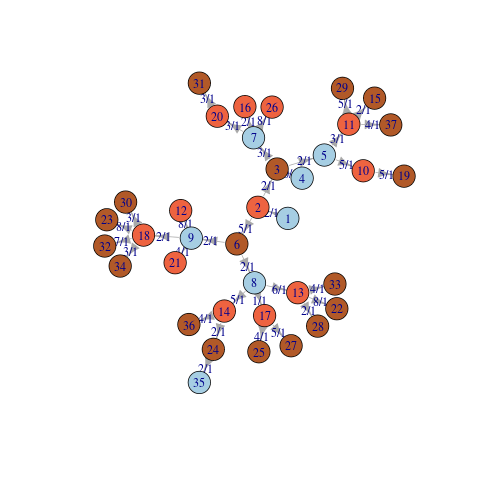
\includegraphics[scale=0.3]{treexample.png} \newline
\caption{{\bf Example transmission tree from simulated outbreak data.} A transmission tree constructed from a randomly generated outbreak using the group transmission probability matrix defined in section 2.9. The direction of arrows between nodes determines the direction of infection. The nodes are coloured by the group of the individual}
\end{figure}
We can now go on to generate some data to see how the method performs on simulated data with group structure.

\subsection{Simulation 1}
For the first set of simulations we proposed to generate datasets where outbreaker could already infer the majority of correct ancestries, we could then give outbreaker the group data and an uninformative prior on the matrix $M$ and see how well the posterior distributions of the transmission probability parameters capture the group dynamics of the data.

We used an imagined scenario of collecting outbreak data from districts within a city in West Africa during the 2014 Ebola Virus Disease (EVD) outbreak. In \citet{outbrkr} the outbreaker model is able to reconstruct ancestries well in simulated datasets both with fast pathogen evolution and long generation times, hence making an Ebola-like simulation a good choice for this simulation. The study of the outbreak led the \citet{Ebola14} to hypothesise that the initial geographical spread of EVD was in part due to a large amount of population movement between cities in bordering countries. We aimed to recreate such a migration led transmission on a smaller scale between boroughs in a city. We simulated datasets where infected individuals are divided into groups based upon their borough of residence and the probabilities of transmission between groups is dependent on the amount people travelling between the two boroughs. If many people commute between districts A and B regularly then it is more likely that an individual unknowingly infected with EVD will travel from district A to district B (or vice versa) and transmit EVD to the people who live there during their trip. Thus far there is not any evidence that such asymptomatic transmission of Ebola happens but for the purposes of this hypothetical situation this is not a major concern. To make the scenario as realistic as possible  we used the estimated epidemiological properties of EVD estimated during the recent analysis by \citet{Ebola14}, a full description of the parameter values used can be found in Table 2.1.

\begin{table}[h!]
\centering
{\bf Table of pathogen parameters for simulation 1}
\caption{The table shows the values of the epidemiological properties of the pathogen used in the {\tt simOutbreak} function, the right hand column shows the source from which the parameter value was taken.}
\begin{tabular}{| l | p{4cm} | p{4cm} |}
\hline
Parameter & Value & Source \\
\hline
Generation Time & Gamma distribution with mean = 13.5 days, s.d. = 9.2 days & \citet{Ebola14} \\
\hline
$R0$ & 2.1, close to WHOERT estimate & \citet{Ebola14} \\
\hline
Mutation Rates & Substitution rate per site per day =  5.479452e-06 & \citet{Gire14} \\
\hline
Sequence Length & 19000 bases & \citet{Volchkov99} \\
\hline
\end{tabular}
\end{table}

We also provided {\tt simOutbreak} with further simulation parameters that would characterise the outbreak which we would then analyse with outbreaker, a full description of these parameters can be found in Table 2.2.
\begin{table}[h!]
\centering
{\bf Table of {\tt simOutbreak} parameters used in simulation 1}
\caption{The table shows the values of the parameters passed to the {\tt simOutbreak} function to simulate outbreak datasets}
\begin{tabular}{|l|l|}
\hline
Parameter & Value \\
\hline
Number of groups & 4 \\
\hline
Group sizes (number of hosts) & 75,75,25,25 (=200) \\
\hline
Group transition matrix &  
$
\begin{pmatrix}
	0.65 & 0.1 & 0.15 & 0.1 \\
	0.1 & 0.6 & 0.1 & 0.2 \\
	0.05 & 0.15 & 0.4 & 0.4 \\
	0.15 & 0.05 & 0.4 & 0.4 \\
\end{pmatrix}
$ \\
\hline
Duration & 50 days \\
\hline
Spatial & FALSE \\
\hline
Number of Iterations and Burn-in & 1e5,2e4 \\
\hline
\end{tabular}
\end{table}

We simulated 440 datasets using these parameters and collected the results from each run of outbreaker on each dataset using a high-performance cluster. Outbreaker was run 4 times on each dataset. One run included both group and DNA sequence data, one run included only group data, one run included only DNA sequence data, and one run included neither types of data (leaving just symptom onset times). All runs were computed for 100000 iterations with a 20000 iteration burn-in period. I discarded 14 datasets where there was not at least one case from each group in the outbreak leaving 426 datasets and their corresponding results. For each dataset we calculated the proportion of consensus ancestries from the posterior tree samples (for all 4 outbreaker runs) that were equal to the real ancestries from the dataset. A consensus ancestry for an individual $i$ is formed by looking for the most common infector of $i$ from the posterior tree samples, the function {\tt get.tTree} in the outbreaker R package performs this task. This check gives some indication that outbreaker was adequately reconstructing the outbreaks.

After this ``sanity test'' assessment we examined the posterior density samples for the transmission probability parameters. Each simulation was generated using the same transmission probability matrix but the number of cases varied so the simulations as a whole should give a good idea of how well the parameters are inferred in for this simulation scenario. Our first step in evaluating the posterior samples for each run was to check whether the true parameter value (used to generate the dataset) fell inside the 95\% equal-tails interval (a credible interval with 2.5\% of the posterior density in each tail). I then counted how many times this occurred for each parameter over all of the simulations to quantify how often outbreaker infers a posterior distribution with a reasonable probability of giving the true parameter value.
\subsection{Simulation 2}
We also hoped to show that the group likelihood could help to infer correct ancestries in situations where the genetic and epidemiological likelihoods were not so effective. These situations are characterised by an outbreak where there are low rates mutation in the pathogen DNA sequences and a fairly flat pathogen generation time, outbreaker struggles with outbreak reconstruction under these conditions \citep{outbrkr}.  In these situations the original outbreaker model without group data struggles to infer the correct ancestor for two reasons. The genetic likelihood cannot narrow down the ancestor because there are few mutations between cases so most previous cases will have very similar genetic likelihoods. Secondly, the epidemiological likelihood struggles because the fairly long generation time means that for a newly infected case outbreaker has to look quite far back into the past for potential ancestors, this will bring up many candidate ancestors and outbreaker have no other way to determine who the correct ancestor is likely to be. In the schematic example shown in Figure 2.2, if there are not many mutations between cases, outbreaker would have trouble inferring an ancestor out of cases 1 to 5.
\\
\begin{figure}[h!]
\centering
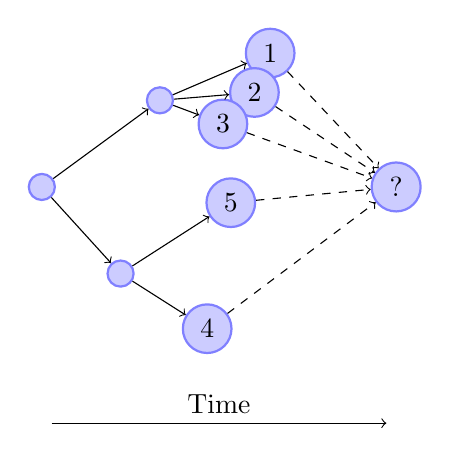
\begin{tikzpicture}
	\node at (0,0) (1){};
	\node at (4.5,0) (2){};
	\node at (0,3) [circle, draw=blue!50, fill=blue!20, thick] (c1) {};
	\node at (1.5,4.1) [circle, draw=blue!50, fill=blue!20, thick] (c2) {};
	\node at (1,1.9) [circle, draw=blue!50, fill=blue!20, thick] (c3) {};
	\node at (2.9,4.7) [circle, draw=blue!50, fill=blue!20, thick] (c4) {1};
	\node at (2.7,4.2) [circle, draw=blue!50, fill=blue!20, thick] (c5) {2};
	\node at (2.3,3.8) [circle, draw=blue!50, fill=blue!20, thick] (c6) {3};	
	\node at (2.1,1.2) [circle, draw=blue!50, fill=blue!20, thick] (c7) {4};
	\node at (2.4,2.8) [circle, draw=blue!50, fill=blue!20, thick] (c8) {5};		
	\node at (4.5,3) [circle, draw=blue!50, fill=blue!20, thick] (c9) {?};
	\node at (2,2) (3) {};
	\node at (4.5,2) (4) {};
	
	\draw [->] (1) -- (2) node[midway, above] {Time};
	\draw [->] (c1) -- (c2); 
	\draw [->] (c1) -- (c3);
	\draw [->] (c2) -- (c4); 
	\draw [->] (c2) -- (c5); 
	\draw [->] (c2) -- (c6);
	\draw [->] (c3) -- (c7); 
	\draw [->] (c3) -- (c8);
	\draw [->] (c4) -- (c9)[dashed]; 
	\draw [->] (c5) -- (c9)[dashed]; 
	\draw [->] (c6) -- (c9)[dashed];
	\draw [->] (c7) -- (c9)[dashed]; 
	\draw [->] (c8) -- (c9)[dashed];
	
	
	
	 	 			 
\end{tikzpicture} \newline

\caption{{\bf Schematic example of outbreaker model inference without group data}. The figure shows a transmission tree, each node is an infected individual and each full line shows a previously inferred transmission event. The node with a ``?'' is a newly infected case, the dotted lines represent potential infectors of ``?''. The figure aims to show that in this scenario outbreaker would have difficulty inferring the correct infector of ``?''}
\end{figure}
The group likelihood can help in this situation if the cases are divided into groups and we have good information on the group transmission probabilities in this situation are. If we are confident that most transmission takes place within groups we could provide a prior that heavily promotes high within group transmission probabilities and low between groups ones. If the data has a true group structure where transmission happens overwhelmingly within groups this will be inferred quickly by the model because it is encouraged by the prior. Therefore when we go to assess the group likelihood of a particular ancestry, it will give a much higher likelihood value to ancestors within the same group as the infected case. 

Returning to the schematic example now shown in Figure 2.3, if the newly infected case belongs to group A and there are 5 candidate ancestors, one of whom belongs to group A, then the likelihood of the connection between the two cases from group A will be much higher and therefore outbreaker will infer this ancestry. Therefore if our prior knowledge that the transmission rates are very unequal is true then we will have biased outbreaker towards the correct ancestries based on their group membership. This is how the group structure of the data and a strong prior can help outbreaker infer correct ancestries in certain situations where the other data is not as useful. In the transmission tree below the nodes are coloured by group membership. If we are trying to guess an ancestor for the new case and we suspect that most transmission occurs within groups then we would guess node 5. If our prior knowledge is accurate then we are making a sensible guess because it would be most likely to have been node 5 that infected our new case. Adding in a group structure and prior knowledge has helped us infer the correct ancestor.
\begin{figure}[h!]
\centering
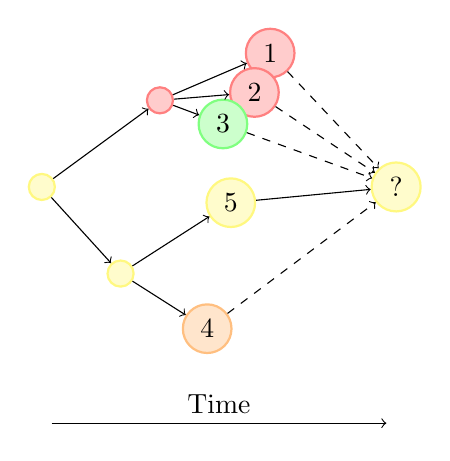
\begin{tikzpicture}
	\node at (0,0) (1){};
	\node at (4.5,0) (2){};
	\node at (0,3) [circle, draw=yellow!50, fill=yellow!20, thick] (c1) {};
	\node at (1.5,4.1) [circle, draw=red!50, fill=red!20, thick] (c2) {};
	\node at (1,1.9) [circle, draw=yellow!50, fill=yellow!20, thick] (c3) {};
	\node at (2.9,4.7) [circle, draw=red!50, fill=red!20, thick] (c4) {1};
	\node at (2.7,4.2) [circle, draw=red!50, fill=red!20, thick] (c5) {2};
	\node at (2.3,3.8) [circle, draw=green!50, fill=green!20, thick] (c6) {3};	
	\node at (2.1,1.2) [circle, draw=orange!50, fill=orange!20, thick] (c7) {4};
	\node at (2.4,2.8) [circle, draw=yellow!50, fill=yellow!20, thick] (c8) {5};		
	\node at (4.5,3) [circle, draw=yellow!50, fill=yellow!20, thick] (c9) {?};
	\node at (2,2) (3) {};
	\node at (4.5,2) (4) {};
	
	\draw [->] (1) -- (2) node[midway, above] {Time};
	\draw [->] (c1) -- (c2); 
	\draw [->] (c1) -- (c3);
	\draw [->] (c2) -- (c4); 
	\draw [->] (c2) -- (c5); 
	\draw [->] (c2) -- (c6);
	\draw [->] (c3) -- (c7); 
	\draw [->] (c3) -- (c8);
	\draw [->] (c4) -- (c9)[dashed]; 
	\draw [->] (c5) -- (c9)[dashed]; 
	\draw [->] (c6) -- (c9)[dashed];
	\draw [->] (c7) -- (c9)[dashed]; 
	\draw [->] (c8) -- (c9);
	
	
	
	 	 			 
\end{tikzpicture}\newline

\caption{{\bf A schematic example of outbreaker model inference with group data.} The figure shows a transmission tree, each node is an infected individual and each full line shows a previous inferred transmission event. Nodes are coloured by their group membership. The node with a ``?'' is a newly infected case, the dotted lines represent potential infectors of ``?''. The figure aims to show that with group data, outbreaker would make the sensible inference that case 5 is the infector of ``?''.}
\end{figure}
To test this, we created a dataset that had small groups containing 3-4 people (households) and one larger group (the community). The true transmission probabilities were designed such that cases within a household had very high probabilities of infecting individuals in the same household, a much lower probability of infecting individuals in the community and an extremely low probability of infecting individuals in other households. Cases in the community had a reasonable probability of infecting others in the community and a relatively low probability of infecting a member from any household. The intention of these groups and parameters was to try and replicate some of the properties of influenza transmission within households that are part of a community \citep{Cauchemez04}. The parameters of the dataset were chosen to provide a balance between an outbreak that the original model would struggle with and an outbreak that resembled an influenza outbreak. Table 2.3 gives the exact parameters given to the {\tt simOutbreak} function to produce this dataset.
\begin{table}[h!]
\centering
{\bf Table of parameters for simulation 2}
\caption{The table gives the values of parameters used to create simulated datasets for simulation 2}
\begin{tabular}{|l|l|}
\hline
Parameter & Value \\
\hline
Generation time & Gamma, mean = 9, s.d = 8.66 (days) \\
\hline
Community group size & 20 \\
\hline
Number of households & 13 = $n_{H}$ \\
\hline
Household sizes & 5,4,6,2,7,6,3,2,3,8,4,2,6 \\
\hline
$R_0$ & 3 \\
\hline
Within household transmission probability & 0.999 $= p_{H}$ \\
\hline
Within community transmission probability & 0.1 $= p_{C}$\\
\hline
Household to community transmission probability & $p_{HtC} =\frac{(1-p_{H})}{2}$ \\
\hline
Community to household transmission probability & $p_{HtH} = \frac{p_{HtC}}{n_{H} - 1}$\\
\hline
DNA sequence mutations per site per day & transitions: 1e-5, transversions: 5e-6 \\
\hline
\end{tabular}
\end{table}
After generating the dataset I performed several runs of outbreaker on it, the first run was the original outbreaker model without group data and the other runs were the extended outbreaker model with a variety of different prior multiplication constants. It is not obvious or easy to find a good value for the multiplication constant so it was decided that we would not try to create run many simulations and perform a systematic analysis. Instead we opted to focus in depth on the results from the single dataset. Further work may be able to determine the properties of a dataset which could inform a sensible prior choice.

We selected the run of the extended outbreaker model which inferred the highest proportion of correct ancestries to compare with the original model. We also looked for the ancestries in each run that had over 75\% support from the estimated posterior distribution. 

\chapter{Results}
\section{Testing Procedures}
In this section we present the results of the two simulations and the analysis of the simulations as described in section 2.9.
\section{Simulation 1: Testing the Ability to Infer Within and Between Group Transmission Probabilities}
First of all the convergence of the Markov chain to the posterior distribution was checked for 10 randomly selected datasets to ascertain that the model with the group data converged to a single distribution and mixed well. An example of one of these MCMC traces is shown in Figure 3.1. The outbreaker runs including group data had uninformative priors that suggested that all group transmission probabilities were equal. 
\begin{figure}
\centering
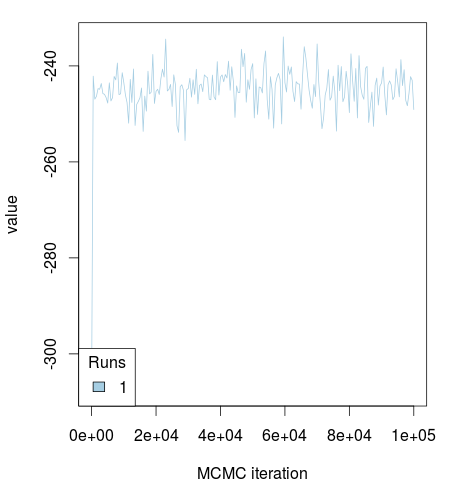
\includegraphics[scale=0.6]{trace.png}
\newline
\caption{{\bf Mixing quality of an extended outbreaker run}. Values of the log-posterior density at every 500 steps of the chain for an example run of the extended outbreaker model on a simulated dataset}
\end{figure}
In line with previous results from \citet{outbrkr} the outbreaker run with group data and DNA sequence data infers a much higher proportion of consensus ancestries that are equal to the real ancestries from the dataset than the outbreaker run with group data and no DNA sequence data. Comparing runs with and without group data also shows that the outbreaker model including the group framework does not seem to perform any different in this scenario. The median proportion of correct consensus ancestries and 95th percentiles of the proportion of correct consensus ancestries for each model, presented by (2.5\% quantile, median, 97.5\% quantile), are as follows: ``all data'', group, DNA sequence and onset times data: (0.553,0.719,0.880); ``dna only'', DNA sequence and onset times data: (0.495,0.697,0.865); ``group only'', group and onset times data: (0.033,0.103,0.229); ``no data'', onset times data only: (0.030,0.086,0.208). This information is displayed graphically in Figure 3.2.
\begin{figure}
\centering
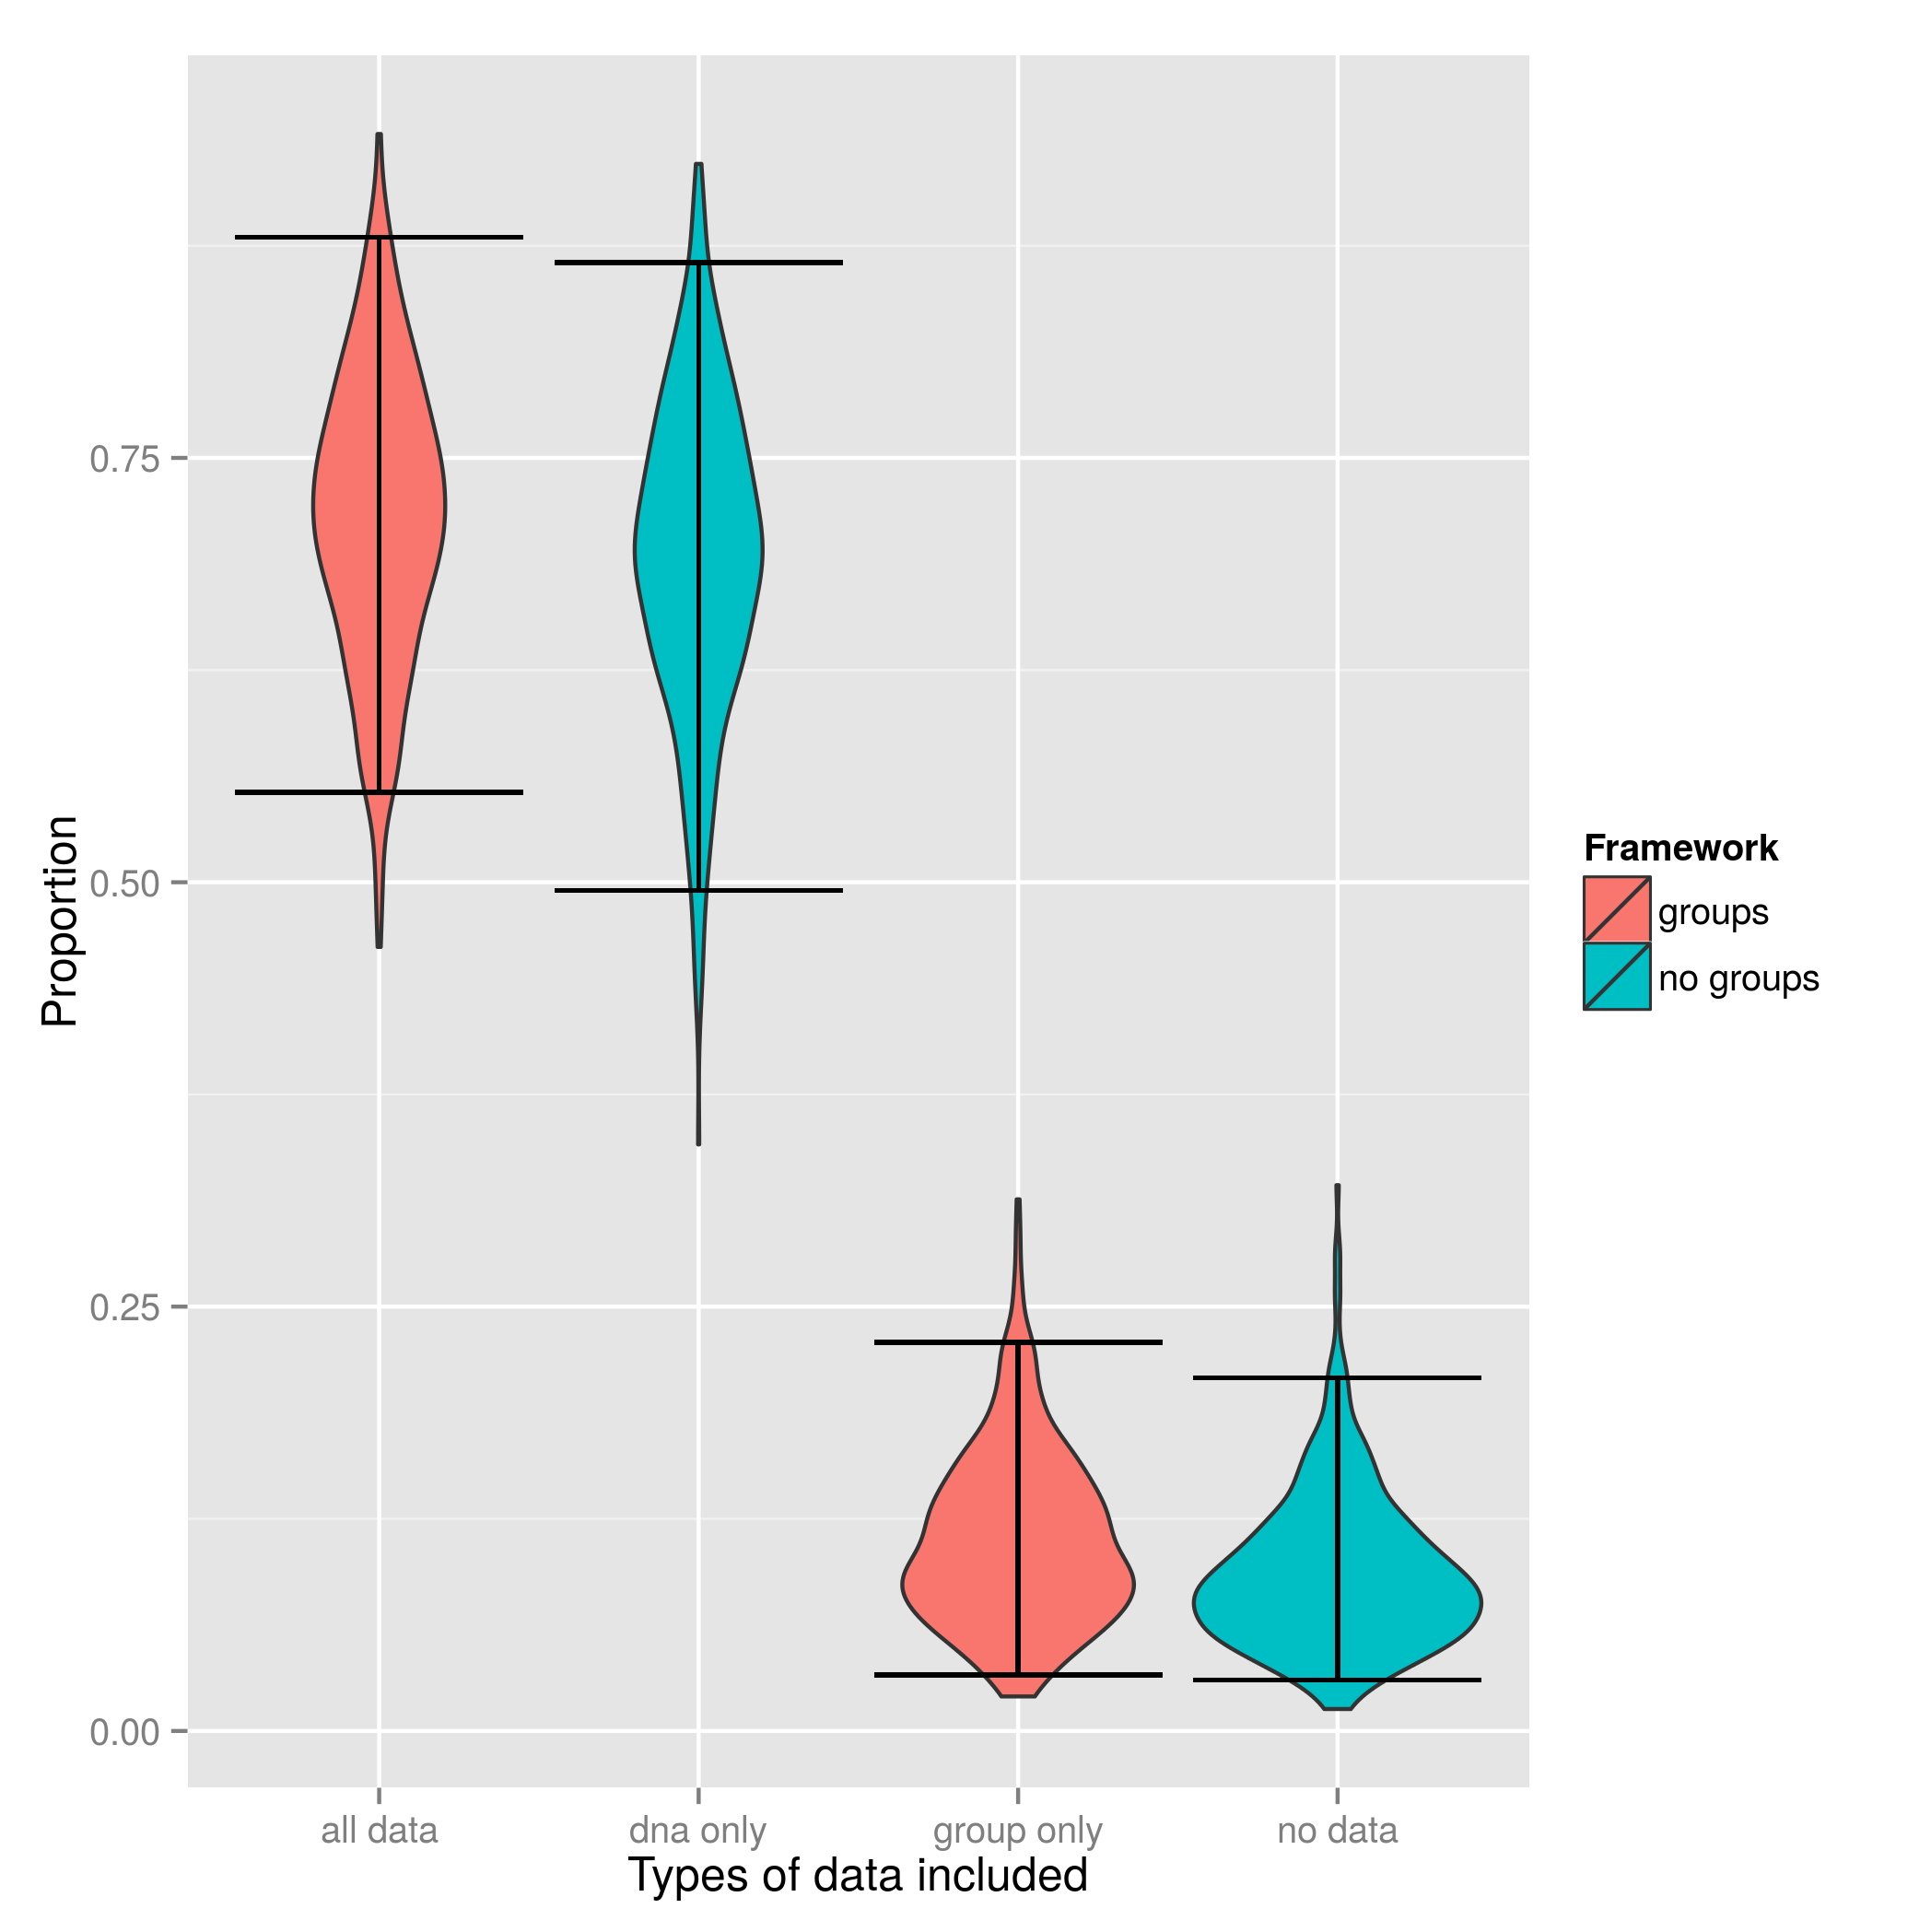
\includegraphics[scale=0.6]{final.png}
\newline
\caption{{\bf Impact of group framework on proportion of correct ancestries inferred}. Violin plot showing the distribution of the proportion of correctly inferred ancestries in the consensus ancestries of outbreaker runs using different versions of the model. The run ``all data'' uses group, DNA and onset time data, the run ``dna only'' uses DNA and onset time data, the run ``group only'' uses group and onset time data and the run ``no data'' uses onset time data only. A consensus ancestry for a case is the most commonly occurring infector in the posterior tree samples, this ancestry is deemed correct if it matches the real ancestry from the dataset. The error bars show where 95\% of the values fell between.}

\end{figure}

We also calculated how many times the outbreaker run including group, DNA and onset times data gave posterior samples for the transmission probability parameters which included the real parameter value in their credible interval. The matrix below shows the corresponding proportion of times that the true transmission probability parameter was within the 95\% equal-tails interval estimated from the posterior samples for that parameter.
\begin{equation}
\begin{pmatrix}
0.8 & 0.87 & 0.97 & 0.99 \\
0.86 & 0.89 & 0.99 & 0.89 \\
0.54 & 0.88 & 0.88 & 0.91 \\
0.89 & 0.48 & 0.91 & 0.87 \\
\end{pmatrix}
\end{equation}

We then studied the variation in the medians of the posterior samples for each parameter across all of the datasets. This gives an indication of confident one should be that the median value of the posterior samples for a transmission probability parameter is close to the real value. See Figure 3.3.
\begin{figure}[h!]
\centering
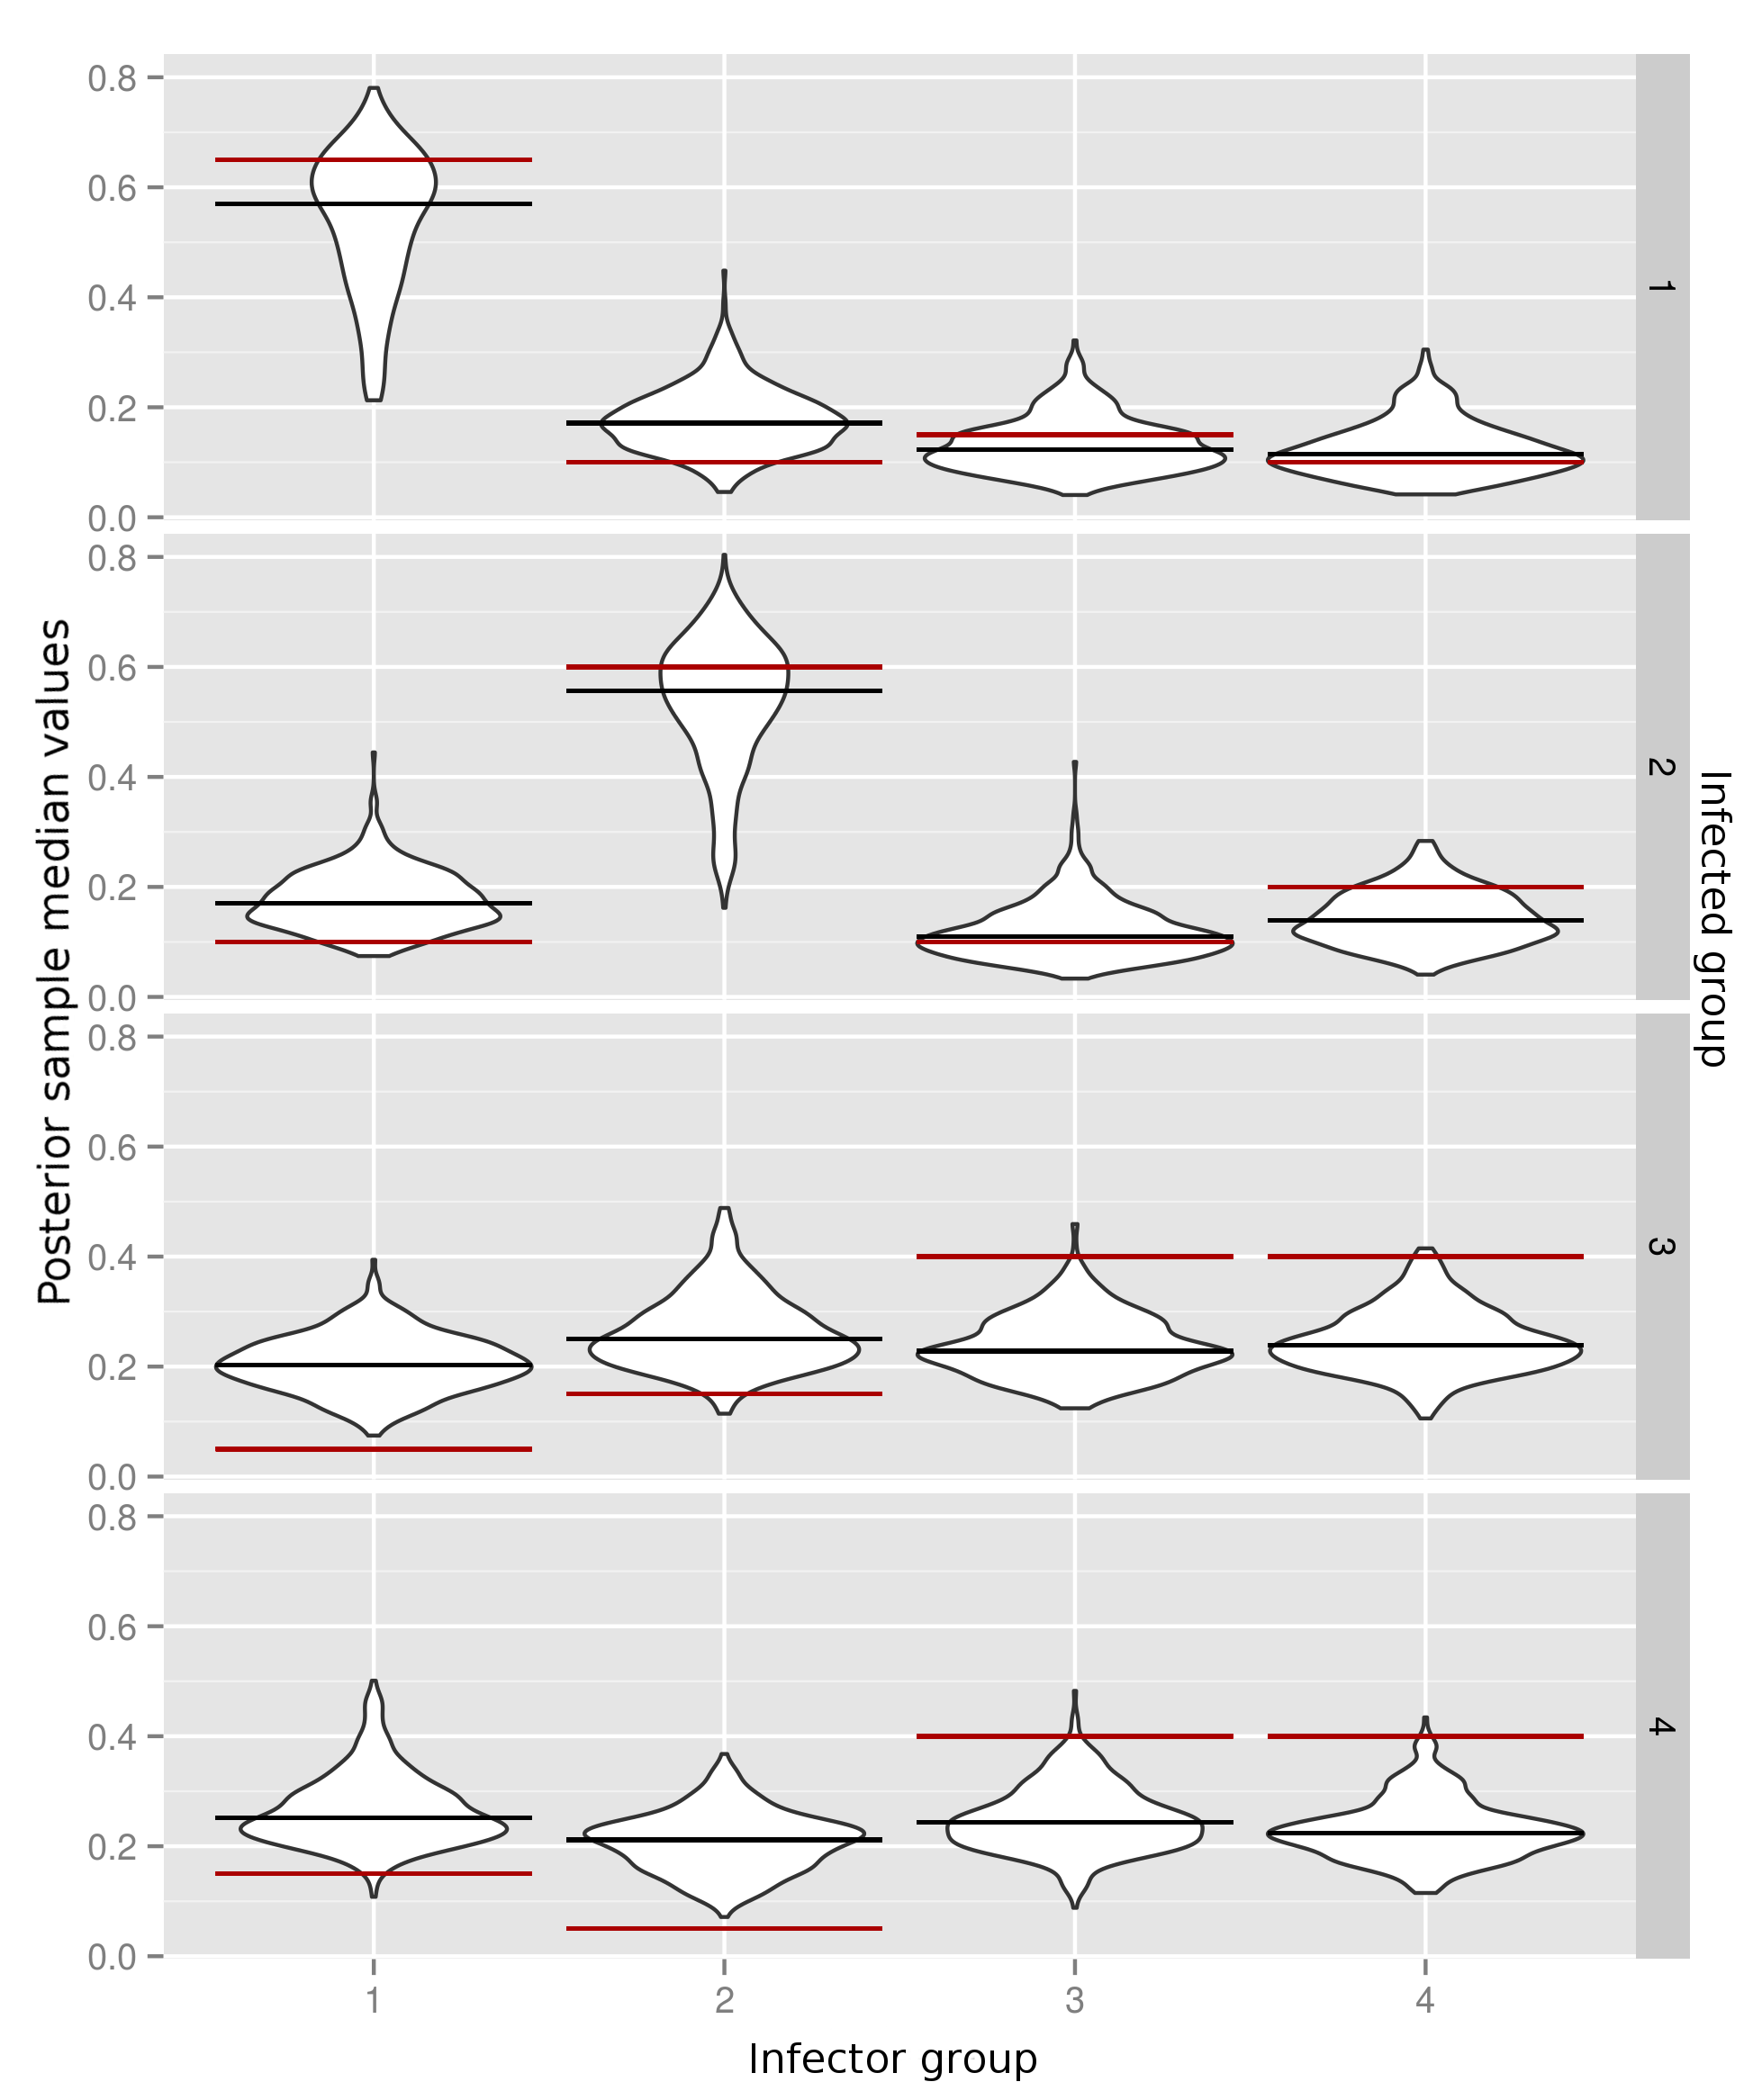
\includegraphics[scale=0.6]{violinmat.png} \newline
\caption{{\bf Variation of posterior sample medians for transmission probability parameters}. Violin plot of the posterior sample medians for each transmission probability parameter. The plot corresponds to the transmission probability matrix containing the true values used in the simulation defined in Table 2.2. Each of the 426 simulations contributes one point (the posterior sample median for that transmission probability parameter) to each of the shapes. The red lines indicate the true values of the parameters used in the simulation and the black lines indicate the median of the posterior medians across all simulations.}
\end{figure}



\section{Simulation 2: Inferring Correct Ancestries}
In this simulation I present the results of the analysis on the dataset simulated using the parameters described in section 2.9.2. The real ancestries from the generated dataset are shown in Figure 3.4, as desired most transmission takes place between members of the same household and the infection mostly moves from household to household via the community. The extended outbreaker run which inferred the highest proportion of correct ancestries had a multiplication constant equal to $0.25$. Figure 3.4 shows the transmission tree of the simulated outbreak. The consensus ancestries inferred by the original outbreaker model with no group data inferred 44 out of 57 ancestry pairs correctly (76\%). The consensus ancestries from the extended model including spatial data inferred 54 out of 57 ancestry pairs correctly (95\%).Figures 3.5 and 3.6 show the consensus ancestries obtained from each run. Strangely both consensus ancestries suggest that cases 53 and 55 infected each other (although this is hard to spot in Figure 3.5).

\begin{figure}
\centering
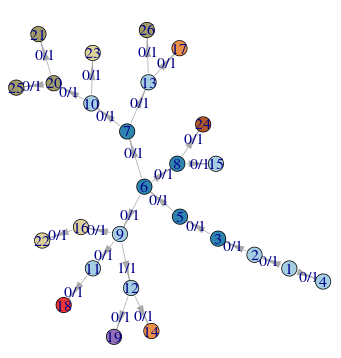
\includegraphics[scale=0.4]{ancestree.png} \newline
\caption{{\bf Transmission tree of real ancestries from simulated dataset}. Transmission tree representing who infected who during simulated outbreak described in sections 3.3 and 4.1.2. Nodes are coloured by their group, the direction of an arrow between two nodes determines the direction of transmission between two individuals. Nodes coloured light blue are members of the community groups, all other coloured nodes are members of one of the 13 households.}
\end{figure}
\begin{figure}[h!]
\centering
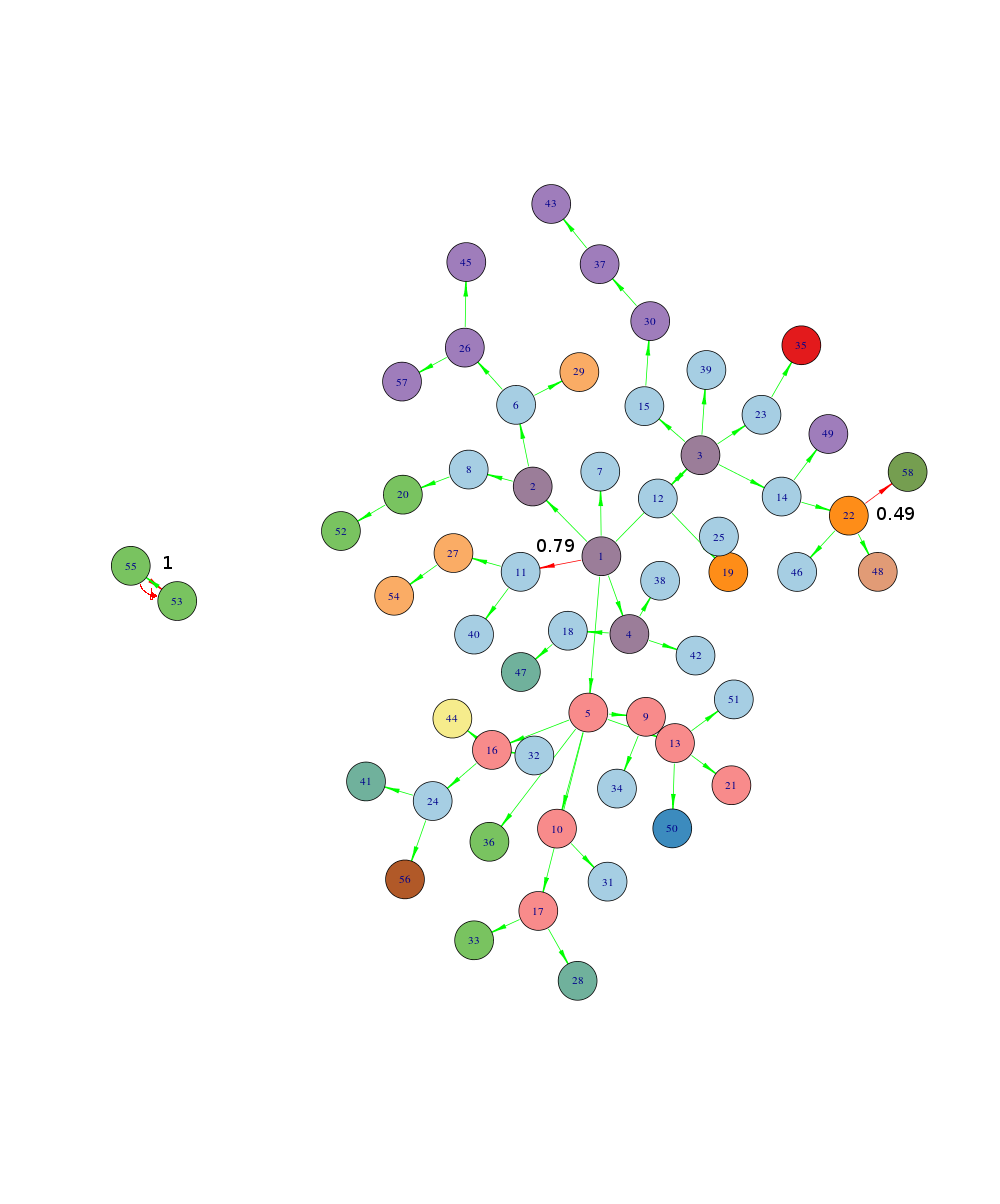
\includegraphics[scale=0.4]{tree_with_grps.png} \newline
\caption{{\bf Transmission tree of consensus ancestries from extended outbreaker model}. Transmission tree inferred by the extended outbreaker model from outbreak data. Nodes are coloured by groups and the direction of arrows between nodes shows the inferred transmission events. Arrows are coloured green if the consensus ancestor is inferred correctly and red otherwise. Nodes coloured light blue are members of the community group, all other coloured nodes are members of one of the 13 households.}
\end{figure}
\begin{figure}[h!]
\centering
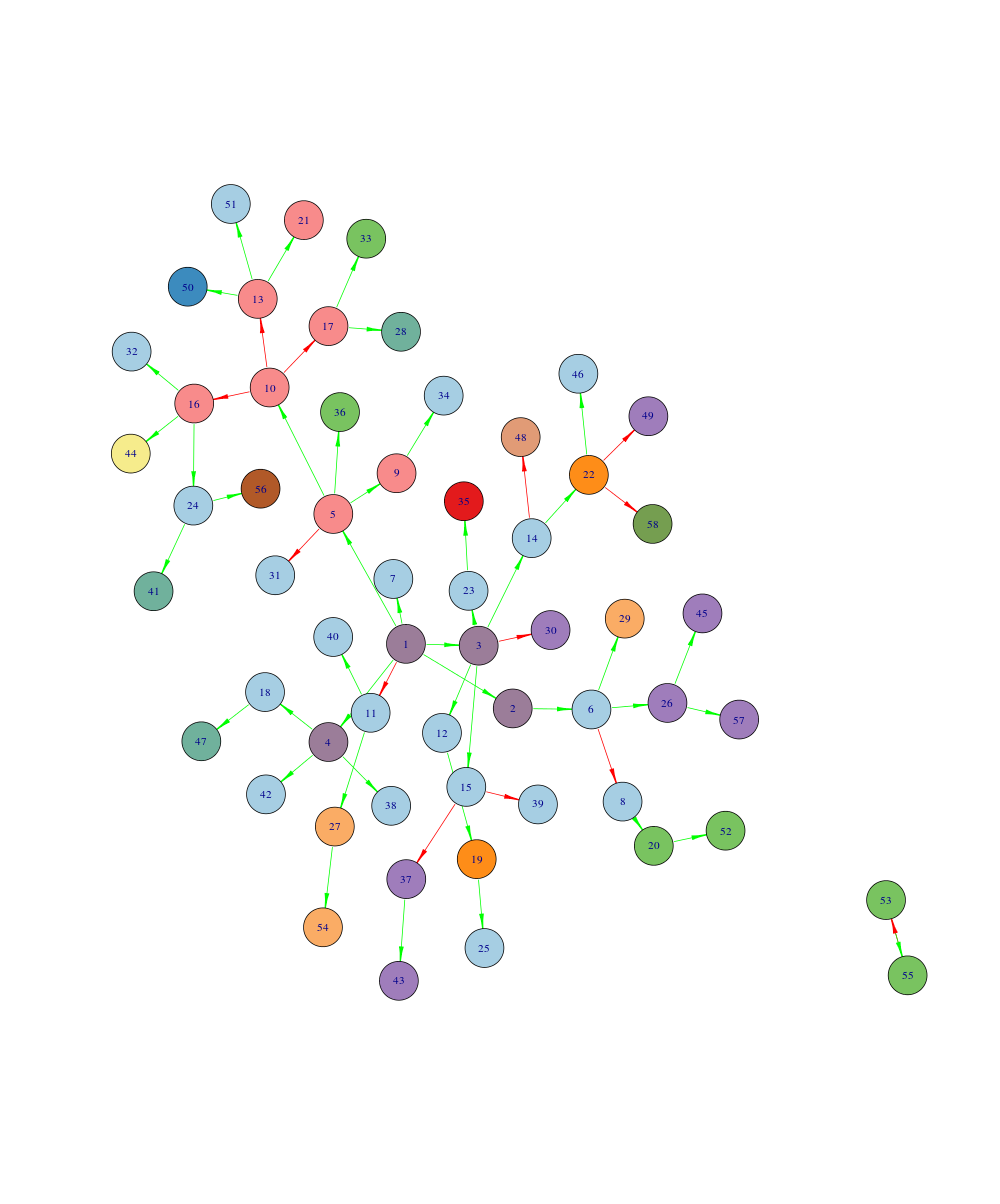
\includegraphics[scale=0.4]{tree_no_grps.png} \newline
\caption{{\bf Transmission tree of consensus ancestries from original outbreaker model (no group framework)}. Transmission tree inferred by the original outbreaker model (no group framework) from outbreak data. Nodes are coloured by groups and the direction of arrows between nodes shows the inferred transmission events. Arrows are coloured green if the consensus ancestor is inferred correctly and red otherwise. Nodes coloured light blue are members of the community group, all other coloured nodes are members of one of the 13 households.}
\end{figure}



\chapter{Discussion}
\section{Results}
\subsection{Estimating Transmission Parameters}
In rows 1 and 2 of Figure 3.3 the medians of the posterior sample medians are closer to the real parameter values used in the simulation than in rows 3 and 4. This suggests that outbreaker infers transmission probability parameters more accurately when one of the parameters in the row is much larger than the others. When there is a strong signal from the group structure of the data, outbreaker is able to provide a reasonable estimation of the true transmission probability parameter from the posterior samples given an uninformative prior. In rows 3 and 4 of Figure 3.3 the medians of the posterior sample medians are around 0.25 suggesting that the within and between group transmission probability parameters are all equal. The uninformative prior used in the simulation hinted that all of the parameters were equal and these results imply that outbreaker did not detect a strong enough signal in the data to move away from this prior assumption about the parameters. 

The matrix (3.1) shows that for the majority of the parameters the 95\% equal-tails interval of the posterior transmission parameter samples included the real parameter value. The two notable cases where this did not happen are elements (3,1) and (4,2) where the real parameter was only in the equal-tails interval around 50\% of the time. These two elements happen to have the smallest real parameter value of 0.05 (see Table 2.2), this seems to show that the model has some difficulty with inferring particularly small transmission probability parameters. Further work to check this interpretation of the results could be to repeat the simulations using different real parameter values for elements (3,2), (3,3) and (3,4) of matrix M to see if the inference of element (3,1) is consistently poor. Another potential area of research would be to repeat the simulation with priors that favour unequal within and between group transmission probabilities to see if this improves the model inference of small transmission parameter values.

For the transmission probability parameters which were greater than 0.05 this is an encouraging sign that the posterior transmission parameter samples from the extended model could be useful for investigating whether within and between group transmission probabilities differ during an outbreak reconstruction. Establishing that most transmission takes place within a certain group could help design intervention methods that target within group transmission, past research on targeted intervention strategies have shown them to be more cost-effective \citep{Lugner13} and to have the potential to improve the disease burden on vulnerable groups \citep{Dushoff07}.  


\subsection{Inferring Correct Ancestries}
For the particular outbreak shown in the results section, adding the group framework to outbreaker greatly improved the proportion of correct ancestries inferred by outbreaker. The benefits of including group data can be seen from the consensus ancestries in the results section, given what we know about the rates of transmission between groups the outbreaker model with the group likelihood produces more sensible results in several cases. The group data has caused outbreaker to infer the correct ancestry between cases 16 and 22, it has also caused outbreaker to guess an ancestry from 16 to 23 which is a sensible inference since it was unlikely that the true ancestry would look as it does with two separate infections of the same household (this is unlikely because households are small relative to the overall population so if two members of a household are infected it is very unlikely that the individual who infected the third member would no be one of the other two members). However, the majority of the ancestries correctly inferred by outbreaker with group data which were not also inferred by outbreaker without group data are transmission events between members of the community and members of households. One explanation for this could be that correct (or more sensible) inferences involving household members elsewhere in the tree made the the correct inferences between individuals 7 and 10 or 7 and 13 more probable.  

\section{Modelling Assumption}
Our model makes some simplifying assumptions which are important to recognise. We must also consider how they may effect the interpretation and usefulness of the model output. The first and main assumption is that the likelihood terms for the genetic, epidemiological and group data are independent. This means that if we choose a candidate ancestry then we expect the values of each of the separate likelihoods not to be correlated. If the pair of cases that we have chosen occur within a short period of time then they would have a high epidemiological likelihood. Due to the short space of time there would not have been many mutations in the DNA sequences of the pathogen, therefore the cases would have a high genetic likelihood. This means that it is unlikely that the values of these two likelihoods would be entirely independent. However, combining these likelihood functions to take account of the correlation would be a very tricky process and would inevitably produce a more complex likelihood function - this has consequences in terms of computational effort when we attempt to compute the likelihood function for thousands of moves during an MCMC run. It is also hard to gauge what sort of effect this assumption will have on the output of the model without computing a combined likelihood and comparing the results.

A second feature of the model is that transmission probabilities between groups are modelled as remaining constant over time. This way of modelling the transmission probabilities serves to constrain the situations in which the extended model would be appropriate. In the two simulation simulations envisioned here it is safe to assume that the transmission rate parameters stay constant during the outbreak because of the 50 day duration of the simulation. Perhaps real data from longer outbreaks with more cases may have heterogeneous group transmission probabilities but large sprawling outbreaks pose other challenges to the outbreaker model such as higher rates of imported and missing cases which also effect the usefulness of the model. One use of the extended model this does rule out is to assess the effectiveness of an intervention on an outbreak (particularly a targeted intervention) because we would expect that interventions might cause the within and between group transmission probabilities to change over time. However, data from two outbreaks that are similar in every other respect apart from the presence of an intervention strategy during one of the outbreaks could be used to compare the effectiveness of the intervention strategy by studying the group transmission probabilities in each case.


\section{Perspectives}
In conclusion, the addition of group data to the outbreaker model has shown that it may be useful in the two scenarios we have tested. Firstly, the model has shown that it is able to infer when there are different transmission probabilities within and between groups. This is useful to those who design intervention policies because it allows them to prioritise the intervention towards groups which are most at risk or drive the ongoing infections within a population \citep{Wallinga10,Dushoff07}.


\bibliographystyle{plainnat}
\bibliography{references}

\end{document}